%%%%%%%%%%%%%%%%%%%%%%%%%%%%%%%%%%%%%%%%%%%%%%%%%%%%%%%%%%
% intro.tex
%%%%%%%%%%%%%%%%%%%%%%%%%%%%%%%%%%%%%%%%%%%%%%%%%%%%%%%%%%

As virtual worlds grow more and more complex, virtual reality browsers and engines face bigger challenges. These challenges are centered on performance on one hand (an interactive framerate is always required) and complexity on the other hand (the larger and more articulated a virtual world, the more immersive the experience).

Modern browsers and engines are based on a data-driven architecture; see Figure \ref{fig:data_driven_games} where we report Figure 1 from \cite{SGL}.

\begin{figure*}
\begin{center}
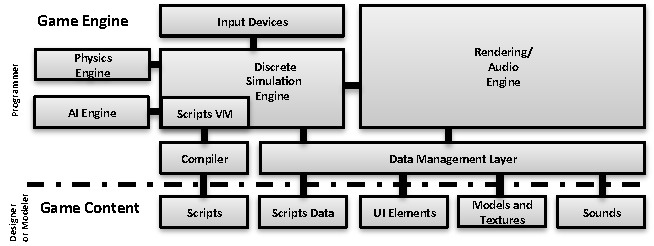
\includegraphics{engine_architecture.pdf}
\end{center}
\label{fig:data_driven_games}
\caption{Data-driven engine architecture}
\end{figure*}

In a data-driven engine the engine contains only general knowledge about virtual worlds, but nothing specific about the virtual world it will animate and render. The specific virtual world will be loaded from the game content in the form of configuration files and scripts. A data-driven engine loads from files two main datasets:

\begin{itemize}
\item a \textbf{scene}, the set of entities that populate the virtual world
\item \textbf{scripts}, the set of (possibly complex) behaviors that animate the scene entities
\end{itemize}

The scene is composed by a heterogeneous set of entities, each of a different kind. Entities may be virtual characters, trees, 2d or 3d models; entities may also be purely logical and invisible such as timers, triggers and proximity sensors.

Scripts are behaviors that animate and give life to these entities by making them ``act'' in an interesting way, either autonomously or reacting to the user's input. Scripts are often divided in two categories: \textbf{reactive} scripts that define simple interactions between pairs of entities and \textbf{behaviors} that define long lasting behaviors such as an AI or the logic according to which a scene keeps generating new entities.

The usual implementation of an engine (see \cite{GAME_OO_HIERARCHY}) features an object-oriented architecture of classes. At the root of this architecture is a class that represents the most generic entity, and from which all other entities are derived. The engine maintains a list of these generic entities, which are all updated and handled through a set of virtual functions. This architecture is a source of often underestimated overhead. Dynamic dispatching is not too costly for a few calls, but when we have many entities, the cost of invoking various virtual functions many times for each frame can become very high. Sometimes the cost of the dynamic dispatching architecture may become higher than the cost of the actual operations being dispatched.

Scripts usually access the scene dynamically. This means that a script must look for the right entities with a mixture of lookups by name and unsafe casts. For example, consider how a Java script may access the \texttt{time} field of a \texttt{myClock} node of type \texttt{timer}:

\begin{lstlisting}
X3DNode myClock = 
 mainScene.getNamedNode("myClock");
SFTime time = 
  (SFTime) myClock.getField("time");
\end{lstlisting}

This style is unsafe, since \texttt{myClock} may not exist or it may have the wrong type, and it also incurs in significant overhead.

In this paper we discuss how we have tackled the problem of increasing performance in X3D browsers while also making scripts safe. We have used a simple compilation technique that removes many unnecessary dynamically dispatched invocations; this technique also allows us to introduce safety for scripts that access the state, so that they do not need to perform unsafe dynamic lookups when searching for specific nodes.

In Section \ref{sec:solution_workflow} we discuss the general shape of our system. In Section \ref{sec:compiling_scene} we show how our technique generates the code and thetype definitions that represent a scene. In Section \ref{sec:compiling_scripts} we discuss how we represent scripts that externally access the scene. In Section \ref{sec:case_study} we show an example of a compiled scene. In Section \ref{sec:benchmarks} we report some benchmarks that show the speedup of using our technique on a sample scene.

\subsection{Related Work}
To the best of our knowledge, this is the first approach that experiments with compiling X3D scripts and scenes in order to achieve greater performance and safe scripts.

Similar, previous approaches towards extending the X3D standard in order to integrate new nodes that support additional features, such as shaders \cite{X3D_OGL_ES}, humanoid behaviors \cite{BEHAVIOR_3D} or procedural definitions of shapes and volumes \cite{FUNCTION_BASED_X3D, FUNCTION_BASED_HAPTIC_X3D}.

None of these approaches though, focus on compilation as a means to achieve higher performance by reducing overhead and safety by introducing compile-time checks.